% \SetPicSubDir{ch-Rice}
% \SetExpSubDir{ch-Rice}

\chapter{Literature Review}
\label{ch:literature}
In this chapter, we lay out the foundation of blockchains and explore a systematic exposition on their recent progress.
We organize the review based on the abstract layers as classified in Figure~\ref{diagram:intro:arch}, before identifying the research gap. 

\section{Data Model Layer}
There are two data organizations in the blockchains, the unspent transaction output-based (UTXO) and the account-based. Their key difference lies whether systems explicitly maintain the states. we illustrate both schemes in Figure~\ref{diagram:literature:data_model}.

\begin{figure}
    \centering
    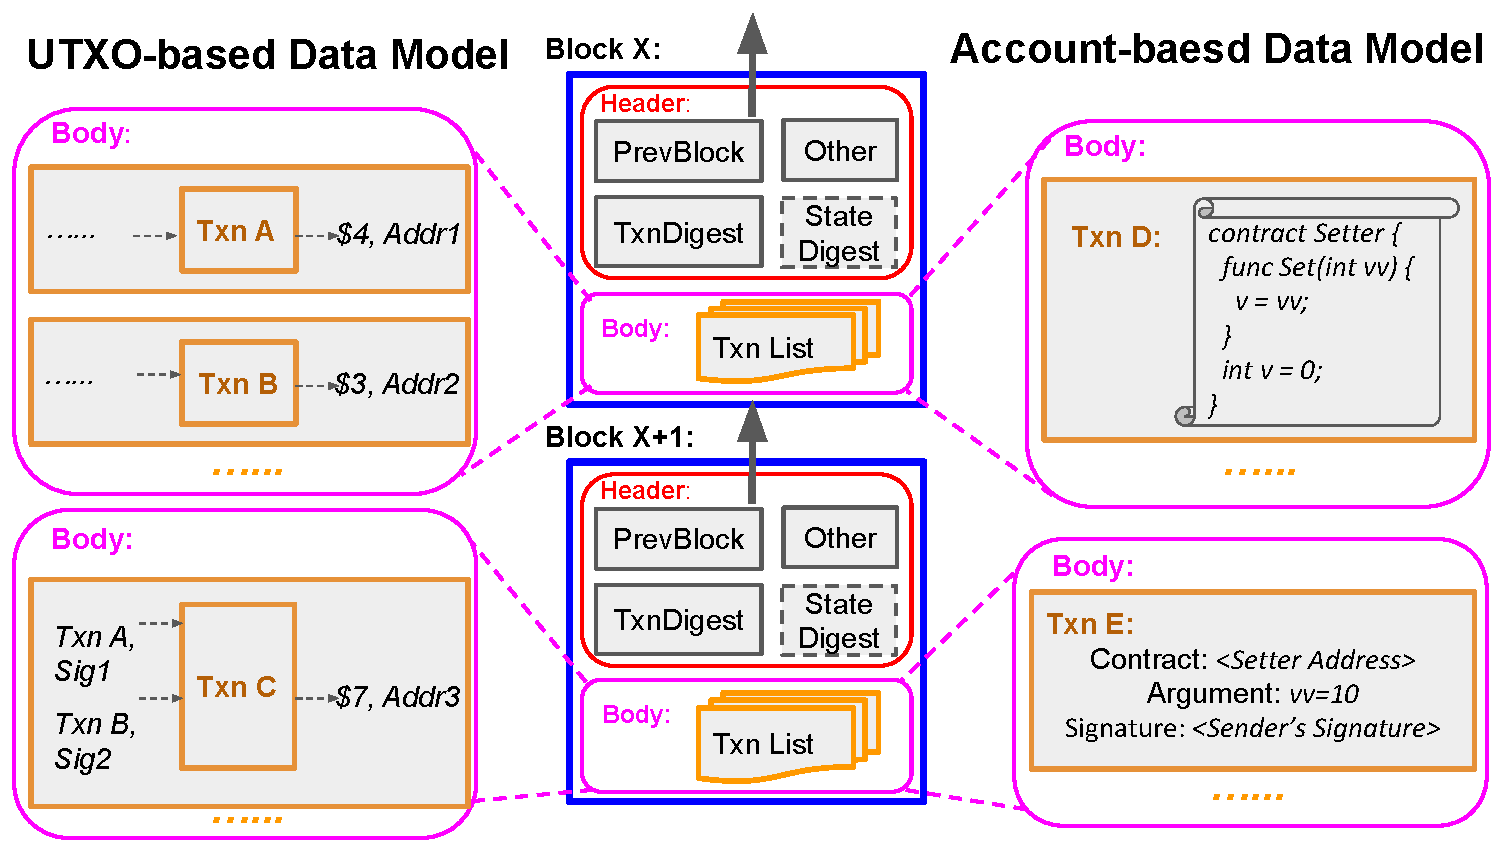
\includegraphics[width=0.8\linewidth]{diagram/literature/data_model.pdf}
    \vspace{\BeforeCaptionVSpace}
    \caption{Unspent Transaction Output (UTXO) and the Account-based data model. }
    \label{diagram:literature:data_model}
\end{figure}

\subsection{UTXO Model}
UTXO purely operates on the transaction basis. In their structure, a transaction consists of multiple inputs and outputs. Each output is associated with an amount of cryptocurrency and an unanswered cryptographic puzzle. Any future transaction can reclaim this amount in its input, by providing the puzzle answer and referencing the previously unspent output. An canonical puzzle and its solution can be an address in the format of a public key hash, and a digital signature from the corresponding private key. Notably, the UTXO model does not bookkeep the balance to addresses. All transactions in the ledger form a Direct Acyclic Graph that records the cryptocurrency flow, where identity hides under the anonymous addresses. 

Bitcoins, due to its decentralization and anonymity, provide a terrain for financial crimes, such as drug dealing and the money laundry. There are a number of attempts to exploit the transactional graph, and identify the pattern for the detection~\cite{fleder2015bitcoin,ron2013quantitative,weber2019anti}. 
Some analysis relies on the graph linkage to discover the identity~\cite{ober2013structure,gaihre2018bitcoin,moser2013anonymity} or other information to predict the bitcoin price~\cite{greaves2015using}. 

\subsection{Account-based Model}
Despite its simplicity, the UTXO model is solely applicable to cryptocurrency-based platforms. 
To support more general workloads, Ethereum introduces the smart contract to encode Turing-complete logic. 
In their design, a transaction either takes in the form of a contract deployment with the executable code. 
Or a transaction provides the execution context to invoke a contract. 
In all cases, each transaction is tagged with the digital signature of the sender. 
In addition, each blockchain peer must explicitly compute for contract states, including the cryptocurrency balance, in each account. 
Such requirement is enforced by the blockchain protocol that all peers shall reach consensus on a post-execution state digest in the block header. 
In contrast, the UTXO-based blockchain only requires for a digest on the transaction integrity.

The account-based data model with smart contracts transition a blockchain into a more general processing platform. 
But it inevitably incurs more vulnerability from the additional complexity. 
For example, some malicious users might run an infinite loop in a transaction to waste system resources. 
To defer such Denial-of-service Attack in the permissionless setting, all blockchains are designed with an incentive-compatible mechanism to prevent the abusive usage. 
For example, Ethereum charges transaction senders with the transaction fee, in a n amount proportional to the number and the complexity of contract operations~\cite{wood2014ethereum}.
Despite this, computational-heavy transactions may still render blockchains securely-flawed: some researchers reveal that rational block validators tend to skip their execution to gain an edge for the next block mining~\cite{luu2015demystifying}.
It is because all the transaction fee is credited to the block miner. 

\section{Execution Layer}
The execution layer concerns on how to process transactions. 
Different blockchain platforms adopt their distinct execution platforms, such as the Docker environment for Hyperledger Fabric and Ethereum Virtual Machine (EVM) for Quorum. 
Despite their implementation differences, the execution architecture of any blockchains falls into either of the following categories. Figure~\ref{diagram:literature:execution} presents their distinction. 

\begin{figure}
    \centering
    \begin{subfigure}{0.95\textwidth}
      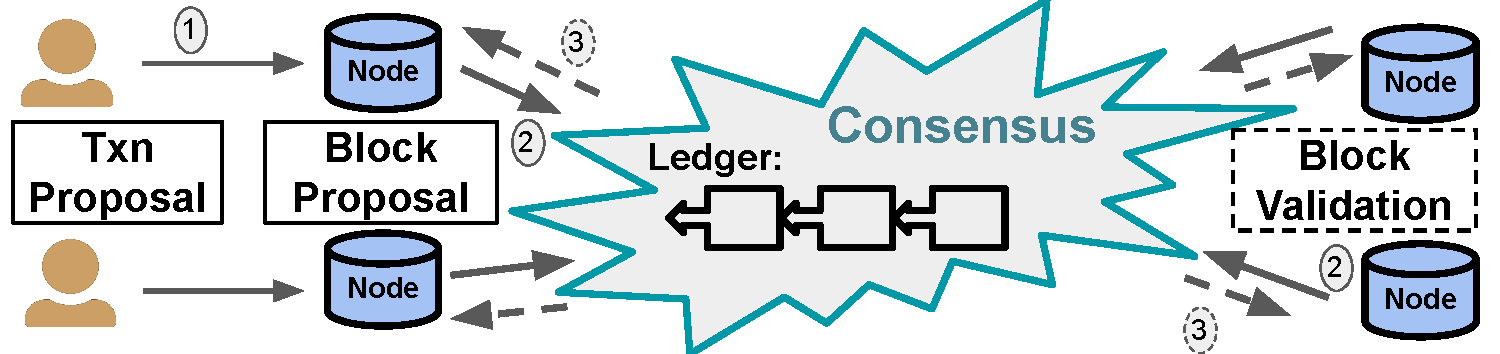
\includegraphics[width=0.99\textwidth]{diagram/literature/ox_arch.pdf}
    \end{subfigure}
    \begin{subfigure}{0.95\textwidth}
      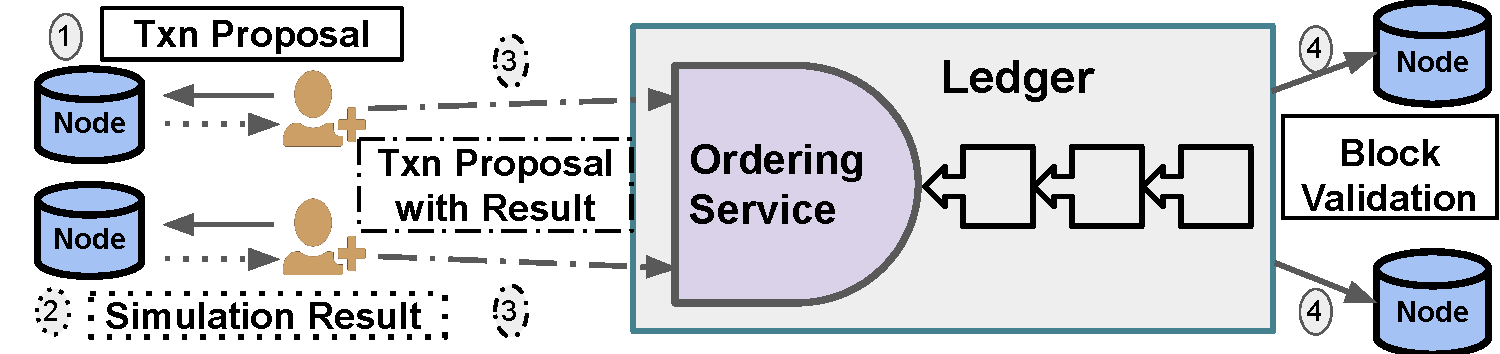
\includegraphics[width=0.99\textwidth]{diagram/literature/eov_arch.pdf}
    \end{subfigure}
    \caption{Comparison of  Order-execute and Execute-order-validate architecture. }
    \label{diagram:literature:execution}
    % \vspace{-1.0em}
\end{figure}

\subsection{Order-execute Architecture}
In the Order-execute architecture, each peer serially executes transactions, based on the established order according to the ledger by the consensus. 
Bitcoin as well as all cryptocurrency-based blockchain adopts this concurrency-free design, simply because the consensus, rather than the execution layer, decides on the system performance. 
Moreover, sequentiality makes it easy to reason about the transaction behavior. 

Despite this, things still get convoluted when transactions deal with Turing-complete logic. For example, many security researchers have demonstrated that Solidity contracts in Ethereum are far more tricky than expected~\cite{luu2016making,parizi2018smart,atzei2017survey}. 
Due to some subtle misunderstanding on operation semantics on EVM, flawed contracts can be exploited by adversaries to gain profits. 
And the problem is further exaggerated given the transparency and the irreversibility of blockchains. 
The concrete DAO hack shows that such an attack is not only a possibility in the theory but a true threat in reality finley201650. 
In the meantime, there come along a series of empirical guidelines and practical tools to aid the contract development~\cite{ducasse2019open,jeng2019step,bai2018formal,tikhomirov2018smartcheck}. 

Through the Order-execute architecture takes on the sequential approach, it is never insulated from the concurrency topic. 
For example, after remarking the reminiscence between contract bugs in blockchains and data races in shared-memory programming, researchers propose a novel viewpoint on the security issues of contracts, from the concurrency perspective in distributed computing~\cite{herlihy2019blockchains,sergey2017concurrent}. 
In ~\cite{dickerson2019adding}, researchers explore to tentatively execute transactions in parallel and then fall into serial if encountering a conflict.  
Instead of speeding up the entire system, the goal of the concurrency is to facilitate the block validation, so that validators can gain a competitive edge on the next block mining. 
Quantitative analysis of the transaction graph shows abundant concurrent chances in mainstream blockchains~\cite{reijsbergen2020exploiting,saraph2019empirical}. 

\subsection{Execute-order-validate Architecture}
Execute-order-validate architecture is proposed in Hyperledger Fabric v1.0~\cite{androulaki2018hyperledger}. 
Rather than taking a monolithic approach, the system is designed with two types of blockchain nodes: peers which execute smart contracts and validate blocks, and orderers which order transactions. 
A transaction pipeline is divided into three phases. 
In the Execute phase, a client requests a subset of peers to execute the transaction speculatively. 
The client collects the results and signatures from peers and sends them to the orderers. 
In the Order phase, orderers order the transactions and batch them into blocks.
For modularity, orderers do not inspect the transaction details. 
In the Validate phase, each peer pulls blocks from the orderers and independently validates each block before persisting the results. 
The block validation process firstly verifies whether transactions satisfy the endorsement policy, i.e., enough number of peers show the endorsement by their signature. 
Then validation procedure checks for conflicts in the read/write sets for each transaction. 
The invalid transactions will not persist their effects, even though they are part of the ledger. 
Read-only queries only involve the Execute phase. 

This architecture brings additional benefits compared to Order-execute architecture. 
Firstly, the endorsement policy decouples the trust condition of a contract from the consensus. 
For example, a valid transaction may carry the execution results from only one of three peers. 
In contrast, the Order-execute architecture mandates the majority of peers to agree on the contract result. 
Secondly, it preserves confidentiality by restricting the execution to specify peers.
Clients, aware of the results before transactions are effected, can also minimize the uncertainty. 
Lastly, speculative execution at the start fits well for the concurrency.
It greatly facilitates computation-heavy transactions, which would queue up in Order-execute architecture. 

However, such concurrency comes with the cost, which manifests as the aborted transactions for the serializability. 
We have empirically demonstrated that in Figure~\ref{chart:intro:basic} and will elaborate this issue in Chapter~\ref{ch:txn}. 
In light of this, Fabric++ reorders transactions during the Order phase to minimize the abort~\cite{sharma2019blurring}. 
OXII architecture is featured for an additional dependency resolution phase at the start~\cite{amiri2019parblockchain}.
So that it enables for a concurrency-friendly transaction schedule. 
OXII relies on the core assumption that the dependency can be extracted by inspecting the contract codebase. 
In the same spirit, XOX architecture runs a patch-up code to streamline a contended transaction~\cite{gorenflo2020xox}. 
The dependency captured during the transaction execution determines this snippet of code. 


% \subsection{Others}

% \section{Consensus Layer}
% \subsection{PoW and its Variants}

% \subsection{PoW and its Enhancements}

% \subsection{Mining Policy and Incentive Analysis}

% \subsection{Byzantine Fault-tolerant Consensus}

% \subsection{Committee-based Consensus}

% \section{Application Layer}
% \subsection{Industrial Proposals}
% \subsection{Benchmarks and Surveys}
% \subsection{Databases or Blockchains}

% % \section{Preliminaries}

% % \lipsum[5-8]

% % \begin{figure}[!t]
% %   \centering
% %   \includegraphics[width=.5\linewidth]{\Pic{jpg}{rice}}
% %   \vspace{\BeforeCaptionVSpace}
% %   \caption{A bowl of rice.}
% %   \label{Rice:fig:bowl_of_rice}
% % \end{figure}

% % \section{Methodology}

% % \autoref{Rice:fig:bowl_of_rice} shows a bowl of rice. 
% % \autoref{Rice:algo:sample} demonstrates the formatting of pseudo code. 
% % Please carefully check the source files and learn how to use this style. 
% % Importantly:

% % \begin{itemize}
% % \item Always state your input.

% % \item State the output if any. 

% % \item Always number your lines for quick referral.

% % \item Always declare and initialize your local variables. 

% % \item Always use \CMD{\gets} (``$\gets$'') for assignments.
% % %Always use \textbackslash gets for assignments.
% % \end{itemize}

% % \begin{algorithm}[!t]
% % \AlgoFontSize
% % \DontPrintSemicolon

% % \KwGlobal{max. calories of daily intake $\mathcal{C}$}
% % \KwGlobal{calories per bowl of rice $\mathcal{B}$}
% % \BlankLine

% % \SetKwFunction{fEatRice}{EatRice}
% % \SetKwFunction{fDoExercise}{DoExercise}

% % \KwIn{number of bowls of rice $n$}
% % \KwOut{calories intake}
% % \Proc{\fEatRice{$n$}}{
% %   $cal \gets n \times \mathcal{B}$\;
% %   \uIf{$cal \geq \mathcal{C}$}{
% %     \Return $\mathcal{C}$\;
% %   }
% %   \Else{
% %     \Return $cal - \fDoExercise{n}$\;
% %   }
% % }

% % \BlankLine

% % \KwIn{time duration (in minutes) of exercise $t$}
% % \KwOut{calories consumed}
% % \Func{\fDoExercise{$t$}}{
% %   $cal \gets 0$\;
% %   \lFor{$i \gets 1$ \To $t$}{$cal \gets cal + i$}
% %   \Return $cal$\;
% % }

% % \caption{Sample pseudo code of a dummy algorithm.}
% % \label{Rice:algo:sample}
% % \end{algorithm}

% % \section{Evaluation}

% % \lipsum[16-19]

% % % \begin{figure}[!t]
% % %   \centering
% % %   \begin{minipage}[b]{.45\linewidth}
% % %     \centering
% % %     \includegraphics[width=\linewidth]{\Exp{eps}{taste_with_meals}}
% % %     \caption{Taste with meal repetition.}
% % %     \label{Rice:exp:taste_with_meals}
% % %   \end{minipage}
% % %   \hspace*{2em}
% % %   \begin{minipage}[b]{.45\linewidth}
% % %     \centering
% % %     \includegraphics[width=\linewidth]{\Exp{eps}{taste_with_freshness}}
% % %     \caption{Taste with meal freshness.}
% % %     \label{Rice:exp:taste_with_freshness}
% % %   \end{minipage}
% % % \end{figure}

% % \autoref{Rice:exp:taste_with_meals} and \autoref{Rice:exp:taste_with_freshness} show how the taste of rice is affected by meal repetition and freshness respectively. 
% % \lipsum[20]

% % \section{Summary}

% % \lipsum[21]
